\section{Physical Simulation}

\subsection{Dynamics Equations}

We model the robot as an articulated rigid body system in our simulator. We represent the states of the system $(\mathbf{x}, \dot{\mathbf{x}})$ in the generalized coordinate, where $\mathbf{x}$ include the global position $\mathbf{p}$, orientation $\mathbf{r}$ of the root link, and the joint angles $\mathbf{q}$. We solve the governing equations of motion eq.(\ref{eq:robotdynamics}) in the generalized coordinates.

\begin{equation}
\label{eq:robotdynamics}
\mathbf{M}(\mathbf{x})\mathbf{\ddot{x}}+\mathbf{C}(\mathbf{x},\mathbf{\dot{x}})=\mathbf{\tau}+\mathbf{J}^T\mathbf{f}
\end{equation}
where $\mathbf{M}(\mathbf{x})$ is the mass matrix and $\mathbf{C}(\mathbf{x},\mathbf{\dot{x}})$ is the Coriolis and Centrifugal force. $\mathbf{\tau}$ are joint torques exerted by the actuators. $\mathbf{J}$ is the Jacobian matrix and $\mathbf{f}$ is the external contact force, which is computed based on linear complementarity conditions. In our implementation, we use DART to compute the contact force and numerically integrate the system state $(\mathbf{x}, \dot{\mathbf{x}})$ over time.

\subsection{Actuator Model}
\label{sec:motorDynamics}
In character animation, the joint torque $\tau$ is often chosen as the control signal since they can be directly integrated in eq.(\ref{eq:robotdynamics}). However, the control signal for the robot that we use in the experiments is the desired joint angles $\bar{\mathbf{q}}$. Given the difference between the desired and the current angle ${q-\bar{q}}$ of each joint, the servo first maps it to a corresponding power level $U$ that is equivalent to changing the voltage across the motor and the voltage is eventually converted to the joint torque $\tau$ according to the internal actuator dynamics.

\begin{figure}[t]
\centering
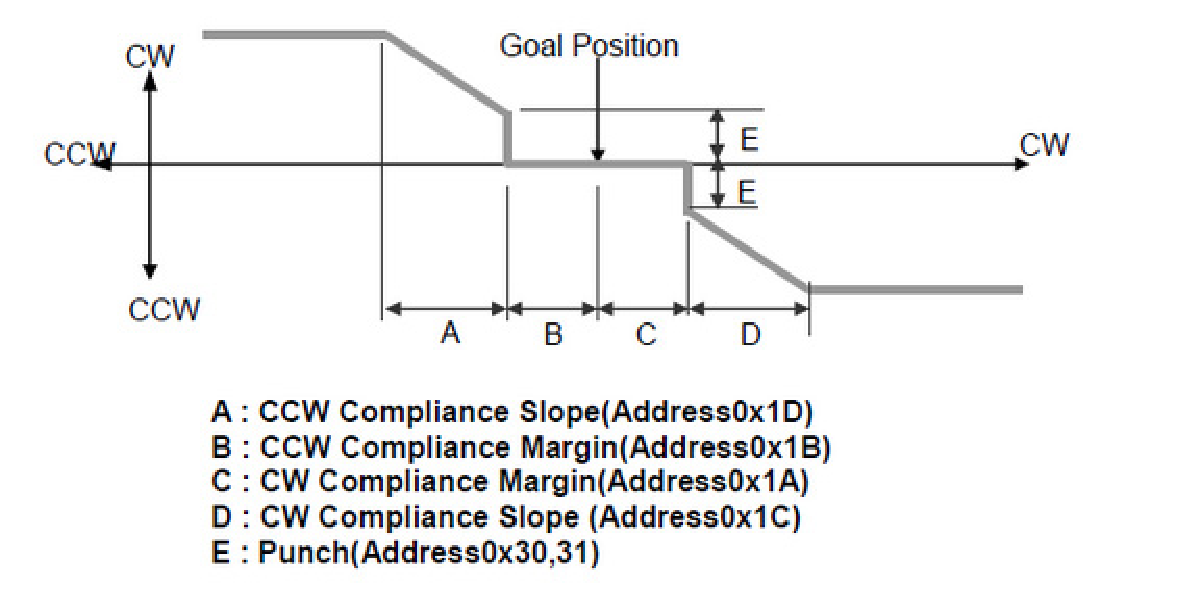
\includegraphics[width=0.45\textwidth]{figures/ax18gain.eps}
\caption{The mapping between $q-\bar{q}$ and $U$ for an AX-18 actuator \cite{AX18:2015}. The x-axis is $q-\bar{q}$ while the y-axis is $U$.}
\label{fig:actuatorMap}
\end{figure}

Most of the actuators on our robot are Dynamixel AX-18, which use the following mapping (Figure \ref{fig:actuatorMap}) between the joint angle difference $q-\bar{q}$ and the power level $U$. The intervals A and D determine the slope of the actuator response for counter-clock-wise and clock-wise motions respectively. Smaller values mean steeper response slopes, in which case the actuator follows the desired angle more closely. However, too small values can lead to overshooting problems. B and C are the compliance margins. If the error of angle is within a small margin specified by B and C, the servo does not output any torque. E, the punch, is the minimum power level before the servo shuts down. In practice, we set A and D to be the same so that the servo will behave the same no matter it rotates clock-wise or counter-clock-wise. In addition, since B, C and E are very small compared to A and D, we ignore their effects and approximate the mapping as linear within the intevals $q-\bar{q}\in A\bigcup B\bigcup C\bigcup D$ with the slope $k_e$:
\begin{equation}
  U=k_e(q-\bar{q})
  \label{eqn:voltageErrorRelation}
\end{equation}

To derive the relation between the power level $U$ and the output torque $\tau$, we adopt a model for the ideal DC motor \cite{SchwarzB:2013}. It is valid to assume an ideal model because the AX-18 servos use high-quality DC motors. The derivation follows by considering the power balance in the motor at a constant voltage U:
\begin{equation}
  P_{electric} = P_{mechanic} + P_{heat}
  \label{eqn:powerBalance}
\end{equation}
where $P_{electric}$ is the electrical power, $P_{mechanic}$ is the mechanical power, and $P_{heat}$ is the power dissipated as heat. From eq.(\ref{eqn:powerBalance}), we can get the following relation:
\begin{equation}
UI=\dot{q}\tau_{motor} + RI^2
\end{equation}
where $I$ is the current and $R$ is the motor winding resistance. In an ideal DC motor, the torque is linearly proportional to the current $\tau_{motor}=k_{\tau}I$. Plugging it into the above equation, we arrive at the relation between the voltage $U$ and the total torque generated by the motor $\tau_{motor}$:
\begin{equation}
  U=k_{\tau}\dot{q}+\frac{R}{k_{\tau}}\tau_{motor}
  \label{eqn:votageTorqueRelation}
\end{equation}
where $k_{\tau}$ is the torque constant, which is determined by the hardware design of the motor. The total torque generated by the motor is not yet the output torque that drives the motor shaft due to the friction inside the motor. The total torque can be decomposed into the output torque $\tau$ and the friction torque $\tau_f$.
\begin{equation}
  \tau_{motor}=\tau+\tau_f
  \label{eqn:torqueBalance}
\end{equation}
The friction torque can be further divided into viscous friction and Coulomb friction \cite{SchwarzB:2013}:
\begin{equation}
  \tau_f = k_v\dot{q}+k_c\sgn(\dot{q})
  \label{eqn:frictionComponents}
\end{equation}
where $k_v$ and $k_c$ are friction coefficients for the viscous and Coulomb friction respectively. $\sgn(x)$ is the sign function that equals 1 if $x$ is positive, -1 if $x$ is negative and 0 otherwise.

Combining eq.(\ref{eqn:votageTorqueRelation}), (\ref{eqn:torqueBalance}) and (\ref{eqn:frictionComponents}), we get the relation between the error of the joint angle $q-\bar{q}$ and the output torque $\tau$.
\begin{align}
\nonumber  \tau & = \frac{k_{\tau}k_e}{R}(q-\bar{q})+(-k_v-\frac{k_{\tau}^2}{R})\dot{q}-k_c\sgn(\dot{q})\\
\nonumber & = -k_p(q-\bar{q}) - k_d\dot{q} - k_c\sgn(\dot{q})\\
  \label{eqn:torqueErrorRelationSimple}
\end{align}
where $k_p=-\frac{k_{\tau}k_e}{R}$ and $k_d=k_v+\frac{k_{\tau}^2}{R}$. We call these values $k_p$, $k_d$ and $k_c$ the \emph{actuator gains}. It is possible to compute these actuator gains if the related parameters are given in the specification sheet of the motor. Plugging eq.(\ref{eqn:torqueErrorRelationSimple}) into (\ref{eq:robotdynamics}), and taking torque limits $[\tau_{min}, \tau_{max}]$ into consideration, we get the dynamics equation that use the desired joint angles as the control signal.
\begin{displaymath}
 \mathbf{M}(\mathbf{x})\mathbf{\ddot{x}}+\mathbf{C}(\mathbf{x},\mathbf{\dot{x}}) = \tau+\mathbf{J}^T\mathbf{f} \\
  \end{displaymath}
where 
\begin{displaymath}\tau =
  \left\{
    \begin{array}{ll}
      \tau_{min} & \text{if }\tau < \tau_{min},\\
      \tau_{max} & \text{if }\tau > \tau_{max},\\
      -k_p(\mathbf{q}-\bar{\mathbf{q}}) - k_d\dot{\mathbf{q}} - k_c\sgn(\dot{\mathbf{q}}) & \text{otherwise.}\\
    \end{array}
  \right.
  \label{eqn:robotDynamicsControl}
\end{displaymath}

\paragraph{Actuator Gain Identification.} We design robot experiments to identify the actuator gains $k_p$, $k_d$ and $k_c$, since the specification of the servos does not provide the necessary information to compute them. In the experiment, we clamp the entire robot on a table except for the left foot. We then send a periodic control signal $\bar{q}(t)$ to the servo at the left ankel (blue curve in Figure \ref{fig:actuatorId} Left). The desired joint angle stays at the maximum value for 0.67 second, then changes to the minimum value and stays for another 0.67 second and repeats. We record the trajectory of the actual joint angle $q(t)$ through the experiment (green curve in Figure \ref{fig:actuatorId} Left). We manually segment out portions of these two curves where the power level is approximately linear to the error $\Delta q = q-\bar{q}$ (the union of intervals A, B, C and D in Figure \ref{fig:actuatorMap}). The black ``+'' in Figure~\ref{fig:actuatorId} Right shows this error over time $\Delta q(t)$ in a typical segment.

\begin{figure}[!t]
  \centering
  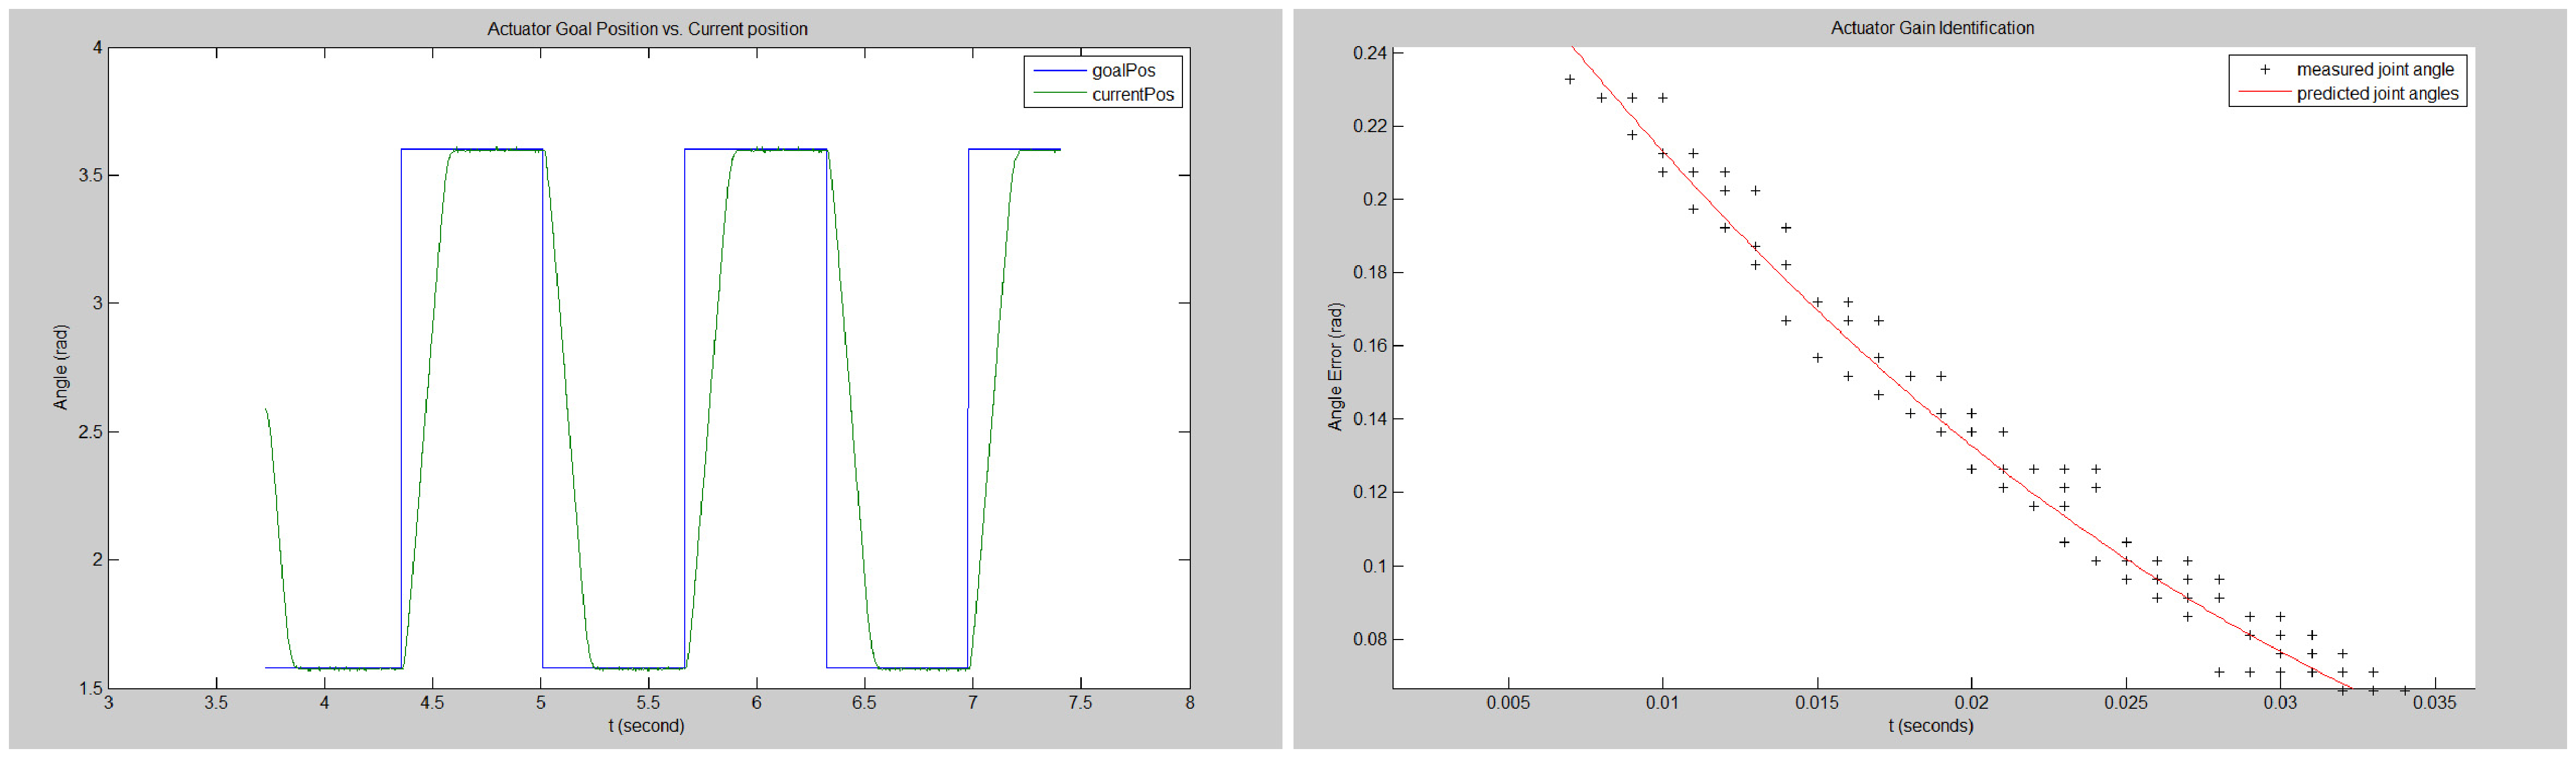
\includegraphics[width=0.5\textwidth]{figures/actuatorId}
  \caption{Actuator Identification. Left: the time series of input desired joint angle and the measured joint angle for an AX-18 servo. Right: the time series of actual error of joint angle and the predicted error using the identified actuator gains.  }
  \label{fig:actuatorId}
\end{figure}

Given $q(t)$ and $\bar{q}(t)$, we can apply regression to estimate the actuator gains. From eq. (\ref{eqn:torqueErrorRelationSimple}), we have
\begin{equation}
\ddot{q}=I^{-1}(-k_p\Delta q - k_d\dot{q} - k_c\sgn(\dot{q}))
\end{equation}
where $I$ is the moment of inertia of the foot with respect to the rotating axis. The above equation is derived by plugging into $\tau = I\ddot{q}+\dot{I}\dot{q}$ and the fact that $\dot{I}\dot{q}=0$ because the foot is a rigid body that rotates along a fixed axis. Ideally, $\ddot{q}$ and $\dot{q}$ can be computed using finite difference. However, the measurement of $q(t)$ is too noisy and finite difference would greatly magnify the noise. To solve this problem, we first smooth $q(t)$ by performing a 4th-order polynomial regression:
\begin{equation}
  \min_{a,b,c,d,e}\int ||q(t)-(at^4+bt^3+ct^2+dt+e)||^2\mathrm{d}t
  \label{eqn:Deltaq}
\end{equation}
where $a,b,c,d,e$ are the polynomial coefficients. This regression gives us a smooth analytical expression of $q(t)$. We then compute $\ddot{q}$ and $\dot{q}$ by differentiate this polynomial analytically:
\begin{align}
\label{eqn:Deltaqdot}  \dot{q}(t)&=4at^3+3bt^2+2ct+d\\
\label{eqn:Deltaqddot}  \ddot{q}(t)&=12at^2+6bt+2c
\end{align}

Combining eq. (\ref{eqn:Deltaq}), (\ref{eqn:Deltaqdot}) and (\ref{eqn:Deltaqddot}), we can perform another regression to compute the actuator gains.
\begin{equation}
\min_{k_p, k_d, k_c}\int||\ddot{q}(t)-I^{-1}(-k_p(q(t)-\bar{q}(t)) - k_d\dot{q}(t) - k_c\sgn(\dot{q}(t)))||^2\mathrm{d}t
\end{equation}

Our experiments and computation show that the actuator gains are $k_p=9.272(N\cdot m/rad)$, $k_d=0.3069(N\cdot m\cdot s/rad)$, and $k_c=0.03(N\cdot m)$. To verify the correctness of these values, we plug them into the simulator and repeat the same experiment in the simulation. The red curve in Figure \ref{fig:actuatorId} Right is the error over time predicted in our simulation, which agrees well with the data that was collected from the robot experiment.

\paragraph{Latency.} To guarantee the stability of the simulation, we use 1ms as the simulation time step. Many animation systems use the same simulation and control frequency, which means that a control signal $\bar{\mathbf{q}}$ is updated every simulation time step. However, the average latency of the whole control loop on our robot is 16ms. It is measured by a timer in our program between the time that the program starts sending the actuator commands to the robot and the time that it finishes reading the sensor measurements from the robot. To better match our simulation with the actual latency, we choose to only update the control signal every 16 time steps.
